\documentclass{article}
\usepackage{graphicx} % Required for inserting images
\usepackage[a4paper, total={6.5 in, 9 in}]{geometry} %this will adjust the height and width of thr height of the text, total={width, height}
\usepackage{amsmath}
\usepackage{times}
\pagestyle{plain}% this will add page nuneber under
\graphicspath{ {images/} }
\usepackage{array,url,kantlipsum}
\newcommand{\Mark}[1]{\textsuperscript{#1}}
\usepackage[font=footnotesize]{caption}
\usepackage{float}
\usepackage{xcolor}
\usepackage{titlesec}
\titlespacing*{\subsubsection}{0pt}{0.1\baselineskip}{0.2\baselineskip}
\usepackage{gensymb}
\titlespacing*{\subsection}{0pt}{0.1\baselineskip}{0.2\baselineskip}

\title{PHY_180_Lab_Report_Reference}
\author{georgexlu.lu }
\date{December 2023}

\begin{document}

\section{}
\section{}
\section{}
\section{}
Part 1 of the results reveals that the period is dependent on the release angle with a quadratic relationship $T = T_0(1 + B\theta_0^2 + C\theta_0^2)$, contradicting predictions of independence. The parameters are $T_0 = 1.13  \pm 1\times10^{-3} $ s $, B = -1.86\times10^{-4}  \pm 7\times10^{-4}$ $\frac{s}{radians}$ $, C = 5.83\times10^{-2} \pm 1\times10^{-3} \frac{s}{radians^2}$. The discrepancies between predictions and observed results can be accounted for by considering uncertainties caused by various physical factors. Notably, when the release angle is below 0.4 radians/22.9 degrees, the period is approximately equal and consistent as the variation in period is well within the error bound of the quadratic function with value of 1.13 seconds.

In Part 2, the Q-factor derived from the simplied exponential model $\theta(t) = \theta_0 e^{-t/\tau}$ equals the one obtained experimentally, falling within the [170,173] range, as their uncertainty ranges overlap. The $\tau$ value for the mathematical model  is $64.3 \pm 2$ and gives a Q-factor of $173 \pm 7$. The Q-factor given by counting method is $170 \pm 6$. This result suggest the mathematical prediction to the relationship between period and Q-factor is fairly accurate. It is also observed that a smaller starting angle gives more accurate Q-factor measurements.

Part 3 of the results show that the period of the pendulum is directly related to the length of the pendulum and can be accurately predicted by the equation $T = KL^n$ with $K = 2.01 \pm 0.01\frac{s}{m^{0.5}}$ and $n = 0.491 \pm 0.01$. The increase in period can be explained by the increase in arc length. As the period is well within the error bound of the exponential function, it can be say that it matches the expect data or the prediction done by the exponential/square root model and proven its viability. 

Part 4 of the results suggest that the Q-factor will decrease as the length increases and can be modeled by the linear function $y = mx + b$ with $m = -225 \pm 18\frac{1}{m}$ and $b = 507 \pm 11$. Since the change in Q-factor is much greater than the uncertainty, it can be said that the parameter is clearly not zero and there is a relation between Q-factor and length. As the Q-values are always well within the error bound, it also proves the reliability of the linear model.

Part 1 of the results reveals that the period is dependent on the release angle with a quadratic relationship $T = T_0(1 + B\theta_0^2 + C\theta_0^2)$, contradicting predictions of independence. The parameters are $T_0 = 1.13  \pm 1\times10^{-3} $ s $, B = -1.86\times10^{-4}  \pm 7\times10^{-4}$ $\frac{s}{radians}$ $, C = 5.83\times10^{-2} \pm 1\times10^{-3} \frac{s}{radians^2}$. The discrepancies between predictions and observed results can be accounted for by considering uncertainties caused by various physical factors. Notably, when the release angle is below 0.4 radians/22.9 degrees, the period is approximately equal and consistent as the variation in period is well within the error bound of the quadratic function with value of 1.13 seconds.

In Part 2, the Q-factor derived from the simplied exponential model $\theta(t) = \theta_0 e^{-t/\tau}$ equals the one obtained experimentally, falling within the [170,173] range, as their uncertainty ranges overlap. The $\tau$ value for the mathematical model  is $64.3 \pm 2$ and gives a Q-factor of $173 \pm 7$. The Q-factor given by counting method is $170 \pm 6$. This result suggest the mathematical prediction to the relationship between period and Q-factor is fairly accurate. It is also observed that a smaller starting angle gives more accurate Q-factor measurements.

Part 3 of the results show that the period of the pendulum is directly related to the length of the pendulum and can be accurately predicted by the equation $T = KL^n$ with $K = 2.01 \pm 0.01\frac{s}{m^{0.5}}$ and $n = 0.491 \pm 0.01$. The increase in period can be explained by the increase in arc length. As the period is well within the error bound of the exponential function, it can be say that it matches the expect data or the prediction done by the exponential/square root model and proven its viability. 

Part 4 of the results suggest that the Q-factor will decrease as the length increases and can be modeled by the linear function $y = mx + b$ with $m = -225 \pm 18\frac{1}{m}$ and $b = 507 \pm 11$. Since the change in Q-factor is much greater than the uncertainty, it can be said that the parameter is clearly not zero and there is a relation between Q-factor and length. As the Q-values are always well within the error bound, it also proves the reliability of the linear model.
Part 1 of the results reveals that the period is dependent on the release angle with a quadratic relationship $T = T_0(1 + B\theta_0^2 + C\theta_0^2)$, contradicting predictions of independence. The parameters are $T_0 = 1.13  \pm 1\times10^{-3} $ s $, B = -1.86\times10^{-4}  \pm 7\times10^{-4}$ $\frac{s}{radians}$ $, C = 5.83\times10^{-2} \pm 1\times10^{-3} \frac{s}{radians^2}$. The discrepancies between predictions and observed results can be accounted for by considering uncertainties caused by various physical factors. Notably, when the release angle is below 0.4 radians/22.9 degrees, the period is approximately equal and consistent as the variation in period is well within the error bound of the quadratic function with value of 1.13 seconds.

In Part 2, the Q-factor derived from the simplied exponential model $\theta(t) = \theta_0 e^{-t/\tau}$ equals the one obtained experimentally, falling within the [170,173] range, as their uncertainty ranges overlap. The $\tau$ value for the mathematical model  is $64.3 \pm 2$ and gives a Q-factor of $173 \pm 7$. The Q-factor given by counting method is $170 \pm 6$. This result suggest the mathematical prediction to the relationship between period and Q-factor is fairly accurate. It is also observed that a smaller starting angle gives more accurate Q-factor measurements.

Part 3 of the results show that the period of the pendulum is directly related to the length of the pendulum and can be accurately predicted by the equation $T = KL^n$ with $K = 2.01 \pm 0.01\frac{s}{m^{0.5}}$ and $n = 0.491 \pm 0.01$. The increase in period can be explained by the increase in arc length. As the period is well within the error bound of the exponential function, it can be say that it matches the expect data or the prediction done by the exponential/square root model and proven its viability. 

Part 4 of the results suggest that the Q-factor will decrease as the length increases and can be modeled by the linear function $y = mx + b$ with $m = -225 \pm 18\frac{1}{m}$ and $b = 507 \pm 11$. Since the change in Q-factor is much greater than the uncertainty, it can be said that the parameter is clearly not zero and there is a relation between Q-factor and length. As the Q-values are always well within the error bound, it also proves the reliability of the linear model.
Part 1 of the results reveals that the period is dependent on the release angle with a quadratic relationship $T = T_0(1 + B\theta_0^2 + C\theta_0^2)$, contradicting predictions of independence. The parameters are $T_0 = 1.13  \pm 1\times10^{-3} $ s $, B = -1.86\times10^{-4}  \pm 7\times10^{-4}$ $\frac{s}{radians}$ $, C = 5.83\times10^{-2} \pm 1\times10^{-3} \frac{s}{radians^2}$. The discrepancies between predictions and observed results can be accounted for by considering uncertainties caused by various physical factors. Notably, when the release angle is below 0.4 radians/22.9 degrees, the period is approximately equal and consistent as the variation in period is well within the error bound of the quadratic function with value of 1.13 seconds.

In Part 2, the Q-factor derived from the simplied exponential model $\theta(t) = \theta_0 e^{-t/\tau}$ equals the one obtained experimentally, falling within the [170,173] range, as their uncertainty ranges overlap. The $\tau$ value for the mathematical model  is $64.3 \pm 2$ and gives a Q-factor of $173 \pm 7$. The Q-factor given by counting method is $170 \pm 6$. This result suggest the mathematical prediction to the relationship between period and Q-factor is fairly accurate. It is also observed that a smaller starting angle gives more accurate Q-factor measurements.

Part 3 of the results show that the period of the pendulum is directly related to the length of the pendulum and can be accurately predicted by the equation $T = KL^n$ with $K = 2.01 \pm 0.01\frac{s}{m^{0.5}}$ and $n = 0.491 \pm 0.01$. The increase in period can be explained by the increase in arc length. As the period is well within the error bound of the exponential function, it can be say that it matches the expect data or the prediction done by the exponential/square root model and proven its viability. 

Part 4 of the results suggest that the Q-factor will decrease as the length increases and can be modeled by the linear function $y = mx + b$ with $m = -225 \pm 18\frac{1}{m}$ and $b = 507 \pm 11$. Since the change in Q-factor is much greater than the uncertainty, it can be said that the parameter is clearly not zero and there is a relation between Q-factor and length. As the Q-values are always well within the error bound, it also proves the reliability of the linear model.
Part 1 of the results reveals that the period is dependent on the release angle with a quadratic relationship $T = T_0(1 + B\theta_0^2 + C\theta_0^2)$, contradicting predictions of independence. The parameters are $T_0 = 1.13  \pm 1\times10^{-3} $ s $, B = -1.86\times10^{-4}  \pm 7\times10^{-4}$ $\frac{s}{radians}$ $, C = 5.83\times10^{-2} \pm 1\times10^{-3} \frac{s}{radians^2}$. The discrepancies between predictions and observed results can be accounted for by considering uncertainties caused by various physical factors. Notably, when the release angle is below 0.4 radians/22.9 degrees, the period is approximately equal and consistent as the variation in period is well within the error bound of the quadratic function with value of 1.13 seconds.

In Part 2, the Q-factor derived from the simplied exponential model $\theta(t) = \theta_0 e^{-t/\tau}$ equals the one obtained experimentally, falling within the [170,173] range, as their uncertainty ranges overlap. The $\tau$ value for the mathematical model  is $64.3 \pm 2$ and gives a Q-factor of $173 \pm 7$. The Q-factor given by counting method is $170 \pm 6$. This result suggest the mathematical prediction to the relationship between period and Q-factor is fairly accurate. It is also observed that a smaller starting angle gives more accurate Q-factor measurements.

Part 3 of the results show that the period of the pendulum is directly related to the length of the pendulum and can be accurately predicted by the equation $T = KL^n$ with $K = 2.01 \pm 0.01\frac{s}{m^{0.5}}$ and $n = 0.491 \pm 0.01$. The increase in period can be explained by the increase in arc length. As the period is well within the error bound of the exponential function, it can be say that it matches the expect data or the prediction done by the exponential/square root model and proven its viability. 

Part 4 of the results suggest that the Q-factor will decrease as the length increases and can be modeled by the linear function $y = mx + b$ with $m = -225 \pm 18\frac{1}{m}$ and $b = 507 \pm 11$. Since the change in Q-factor is much greater than the uncertainty, it can be said that the parameter is clearly not zero and there is a relation between Q-factor and length. As the Q-values are always well within the error bound, it also proves the reliability of the linear model.
Part 1 of the results reveals that the period is dependent on the release angle with a quadratic relationship $T = T_0(1 + B\theta_0^2 + C\theta_0^2)$, contradicting predictions of independence. The parameters are $T_0 = 1.13  \pm 1\times10^{-3} $ s $, B = -1.86\times10^{-4}  \pm 7\times10^{-4}$ $\frac{s}{radians}$ $, C = 5.83\times10^{-2} \pm 1\times10^{-3} \frac{s}{radians^2}$. The discrepancies between predictions and observed results can be accounted for by considering uncertainties caused by various physical factors. Notably, when the release angle is below 0.4 radians/22.9 degrees, the period is approximately equal and consistent as the variation in period is well within the error bound of the quadratic function with value of 1.13 seconds.

In Part 2, the Q-factor derived from the simplied exponential model $\theta(t) = \theta_0 e^{-t/\tau}$ equals the one obtained experimentally, falling within the [170,173] range, as their uncertainty ranges overlap. The $\tau$ value for the mathematical model  is $64.3 \pm 2$ and gives a Q-factor of $173 \pm 7$. The Q-factor given by counting method is $170 \pm 6$. This result suggest the mathematical prediction to the relationship between period and Q-factor is fairly accurate. It is also observed that a smaller starting angle gives more accurate Q-factor measurements.

Part 3 of the results show that the period of the pendulum is directly related to the length of the pendulum and can be accurately predicted by the equation $T = KL^n$ with $K = 2.01 \pm 0.01\frac{s}{m^{0.5}}$ and $n = 0.491 \pm 0.01$. The increase in period can be explained by the increase in arc length. As the period is well within the error bound of the exponential function, it can be say that it matches the expect data or the prediction done by the exponential/square root model and proven its viability. 

Part 4 of the results suggest that the Q-factor will decrease as the length increases and can be modeled by the linear function $y = mx + b$ with $m = -225 \pm 18\frac{1}{m}$ and $b = 507 \pm 11$. Since the change in Q-factor is much greater than the uncertainty, it can be said that the parameter is clearly not zero and there is a relation between Q-factor and length. As the Q-values are always well within the error bound, it also proves the reliability of the linear model.

Part 1 of the results reveals that the period is dependent on the release angle with a quadratic relationship $T = T_0(1 + B\theta_0^2 + C\theta_0^2)$, contradicting predictions of independence. The parameters are $T_0 = 1.13  \pm 1\times10^{-3} $ s $, B = -1.86\times10^{-4}  \pm 7\times10^{-4}$ $\frac{s}{radians}$ $, C = 5.83\times10^{-2} \pm 1\times10^{-3} \frac{s}{radians^2}$. The discrepancies between predictions and observed results can be accounted for by considering uncertainties caused by various physical factors. Notably, when the release angle is below 0.4 radians/22.9 degrees, the period is approximately equal and consistent as the variation in period is well within the error bound of the quadratic function with value of 1.13 seconds.

In Part 2, the Q-factor derived from the simplied exponential model $\theta(t) = \theta_0 e^{-t/\tau}$ equals the one obtained experimentally, falling within the [170,173] range, as their uncertainty ranges overlap. The $\tau$ value for the mathematical model  is $64.3 \pm 2$ and gives a Q-factor of $173 \pm 7$. The Q-factor given by counting method is $170 \pm 6$. This result suggest the mathematical prediction to the relationship between period and Q-factor is fairly accurate. It is also observed that a smaller starting angle gives more accurate Q-factor measurements.

Part 3 of the results show that the period of the pendulum is directly related to the length of the pendulum and can be accurately predicted by the equation $T = KL^n$ with $K = 2.01 \pm 0.01\frac{s}{m^{0.5}}$ and $n = 0.491 \pm 0.01$. The increase in period can be explained by the increase in arc length. As the period is well within the error bound of the exponential function, it can be say that it matches the expect data or the prediction done by the exponential/square root model and proven its viability. 

Part 4 of the results suggest that the Q-factor will decrease as the length increases and can be modeled by the linear function $y = mx + b$ with $m = -225 \pm 18\frac{1}{m}$ and $b = 507 \pm 11$. Since the change in Q-factor is much greater than the uncertainty, it can be said that the parameter is clearly not zero and there is a relation between Q-factor and length. As the Q-values are always well within the error bound, it also proves the reliability of the linear model.

Part 1 of the results reveals that the period is dependent on the release angle with a quadratic relationship $T = T_0(1 + B\theta_0^2 + C\theta_0^2)$, contradicting predictions of independence. The parameters are $T_0 = 1.13  \pm 1\times10^{-3} $ s $, B = -1.86\times10^{-4}  \pm 7\times10^{-4}$ $\frac{s}{radians}$ $, C = 5.83\times10^{-2} \pm 1\times10^{-3} \frac{s}{radians^2}$. The discrepancies between predictions and observed results can be accounted for by considering uncertainties caused by various physical factors. Notably, when the release angle is below 0.4 radians/22.9 degrees, the period is approximately equal and consistent as the variation in period is well within the error bound of the quadratic function with value of 1.13 seconds.

In Part 2, the Q-factor derived from the simplied exponential model $\theta(t) = \theta_0 e^{-t/\tau}$ equals the one obtained experimentally, falling within the [170,173] range, as their uncertainty ranges overlap. The $\tau$ value for the mathematical model  is $64.3 \pm 2$ and gives a Q-factor of $173 \pm 7$. The Q-factor given by counting method is $170 \pm 6$. This result suggest the mathematical prediction to the relationship between period and Q-factor is fairly accurate. It is also observed that a smaller starting angle gives more accurate Q-factor measurements.

Part 3 of the results show that the period of the pendulum is directly related to the length of the pendulum and can be accurately predicted by the equation $T = KL^n$ with $K = 2.01 \pm 0.01\frac{s}{m^{0.5}}$ and $n = 0.491 \pm 0.01$. The increase in period can be explained by the increase in arc length. As the period is well within the error bound of the exponential function, it can be say that it matches the expect data or the prediction done by the exponential/square root model and proven its viability. 

Part 4 of the results suggest that the Q-factor will decrease as the length increases and can be modeled by the linear function $y = mx + b$ with $m = -225 \pm 18\frac{1}{m}$ and $b = 507 \pm 11$. Since the change in Q-factor is much greater than the uncertainty, it can be said that the parameter is clearly not zero and there is a relation between Q-factor and length. As the Q-values are always well within the error bound, it also proves the reliability of the linear model.
Part 1 of the results reveals that the period is dependent on the release angle with a quadratic relationship $T = T_0(1 + B\theta_0^2 + C\theta_0^2)$, contradicting predictions of independence. The parameters are $T_0 = 1.13  \pm 1\times10^{-3} $ s $, B = -1.86\times10^{-4}  \pm 7\times10^{-4}$ $\frac{s}{radians}$ $, C = 5.83\times10^{-2} \pm 1\times10^{-3} \frac{s}{radians^2}$. The discrepancies between predictions and observed results can be accounted for by considering uncertainties caused by various physical factors. Notably, when the release angle is below 0.4 radians/22.9 degrees, the period is approximately equal and consistent as the variation in period is well within the error bound of the quadratic function with value of 1.13 seconds.

In Part 2, the Q-factor derived from the simplied exponential model $\theta(t) = \theta_0 e^{-t/\tau}$ equals the one obtained experimentally, falling within the [170,173] range, as their uncertainty ranges overlap. The $\tau$ value for the mathematical model  is $64.3 \pm 2$ and gives a Q-factor of $173 \pm 7$. The Q-factor given by counting method is $170 \pm 6$. This result suggest the mathematical prediction to the relationship between period and Q-factor is fairly accurate. It is also observed that a smaller starting angle gives more accurate Q-factor measurements.

Part 3 of the results show that the period of the pendulum is directly related to the length of the pendulum and can be accurately predicted by the equation $T = KL^n$ with $K = 2.01 \pm 0.01\frac{s}{m^{0.5}}$ and $n = 0.491 \pm 0.01$. The increase in period can be explained by the increase in arc length. As the period is well within the error bound of the exponential function, it can be say that it matches the expect data or the prediction done by the exponential/square root model and proven its viability. 

Part 4 of the results suggest that the Q-factor will decrease as the length increases and can be modeled by the linear function $y = mx + b$ with $m = -225 \pm 18\frac{1}{m}$ and $b = 507 \pm 11$. Since the change in Q-factor is much greater than the uncertainty, it can be said that the parameter is clearly not zero and there is a relation between Q-factor and length. As the Q-values are always well within the error bound, it also proves the reliability of the linear model.
Part 1 of the results reveals that the period is dependent on the release angle with a quadratic relationship $T = T_0(1 + B\theta_0^2 + C\theta_0^2)$, contradicting predictions of independence. The parameters are $T_0 = 1.13  \pm 1\times10^{-3} $ s $, B = -1.86\times10^{-4}  \pm 7\times10^{-4}$ $\frac{s}{radians}$ $, C = 5.83\times10^{-2} \pm 1\times10^{-3} \frac{s}{radians^2}$. The discrepancies between predictions and observed results can be accounted for by considering uncertainties caused by various physical factors. Notably, when the release angle is below 0.4 radians/22.9 degrees, the period is approximately equal and consistent as the variation in period is well within the error bound of the quadratic function with value of 1.13 seconds.

In Part 2, the Q-factor derived from the simplied exponential model $\theta(t) = \theta_0 e^{-t/\tau}$ equals the one obtained experimentally, falling within the [170,173] range, as their uncertainty ranges overlap. The $\tau$ value for the mathematical model  is $64.3 \pm 2$ and gives a Q-factor of $173 \pm 7$. The Q-factor given by counting method is $170 \pm 6$. This result suggest the mathematical prediction to the relationship between period and Q-factor is fairly accurate. It is also observed that a smaller starting angle gives more accurate Q-factor measurements.

Part 3 of the results show that the period of the pendulum is directly related to the length of the pendulum and can be accurately predicted by the equation $T = KL^n$ with $K = 2.01 \pm 0.01\frac{s}{m^{0.5}}$ and $n = 0.491 \pm 0.01$. The increase in period can be explained by the increase in arc length. As the period is well within the error bound of the exponential function, it can be say that it matches the expect data or the prediction done by the exponential/square root model and proven its viability. 

Part 4 of the results suggest that the Q-factor will decrease as the length increases and can be modeled by the linear function $y = mx + b$ with $m = -225 \pm 18\frac{1}{m}$ and $b = 507 \pm 11$. Since the change in Q-factor is much greater than the uncertainty, it can be said that the parameter is clearly not zero and there is a relation between Q-factor and length. As the Q-values are always well within the error bound, it also proves the reliability of the linear model.
Part 1 of the results reveals that the period is dependent on the release angle with a quadratic relationship $T = T_0(1 + B\theta_0^2 + C\theta_0^2)$, contradicting predictions of independence. The parameters are $T_0 = 1.13  \pm 1\times10^{-3} $ s $, B = -1.86\times10^{-4}  \pm 7\times10^{-4}$ $\frac{s}{radians}$ $, C = 5.83\times10^{-2} \pm 1\times10^{-3} \frac{s}{radians^2}$. The discrepancies between predictions and observed results can be accounted for by considering uncertainties caused by various physical factors. Notably, when the release angle is below 0.4 radians/22.9 degrees, the period is approximately equal and consistent as the variation in period is well within the error bound of the quadratic function with value of 1.13 seconds.

In Part 2, the Q-factor derived from the simplied exponential model $\theta(t) = \theta_0 e^{-t/\tau}$ equals the one obtained experimentally, falling within the [170,173] range, as their uncertainty ranges overlap. The $\tau$ value for the mathematical model  is $64.3 \pm 2$ and gives a Q-factor of $173 \pm 7$. The Q-factor given by counting method is $170 \pm 6$. This result suggest the mathematical prediction to the relationship between period and Q-factor is fairly accurate. It is also observed that a smaller starting angle gives more accurate Q-factor measurements.

Part 3 of the results show that the period of the pendulum is directly related to the length of the pendulum and can be accurately predicted by the equation $T = KL^n$ with $K = 2.01 \pm 0.01\frac{s}{m^{0.5}}$ and $n = 0.491 \pm 0.01$. The increase in period can be explained by the increase in arc length. As the period is well within the error bound of the exponential function, it can be say that it matches the expect data or the prediction done by the exponential/square root model and proven its viability. 

Part 4 of the results suggest that the Q-factor will decrease as the length increases and can be modeled by the linear function $y = mx + b$ with $m = -225 \pm 18\frac{1}{m}$ and $b = 507 \pm 11$. Since the change in Q-factor is much greater than the uncertainty, it can be said that the parameter is clearly not zero and there is a relation between Q-factor and length. As the Q-values are always well within the error bound, it also proves the reliability of the linear model.
Part 1 of the results reveals that the period is dependent on the release angle with a quadratic relationship $T = T_0(1 + B\theta_0^2 + C\theta_0^2)$, contradicting predictions of independence. The parameters are $T_0 = 1.13  \pm 1\times10^{-3} $ s $, B = -1.86\times10^{-4}  \pm 7\times10^{-4}$ $\frac{s}{radians}$ $, C = 5.83\times10^{-2} \pm 1\times10^{-3} \frac{s}{radians^2}$. The discrepancies between predictions and observed results can be accounted for by considering uncertainties caused by various physical factors. Notably, when the release angle is below 0.4 radians/22.9 degrees, the period is approximately equal and consistent as the variation in period is well within the error bound of the quadratic function with value of 1.13 seconds.

In Part 2, the Q-factor derived from the simplied exponential model $\theta(t) = \theta_0 e^{-t/\tau}$ equals the one obtained experimentally, falling within the [170,173] range, as their uncertainty ranges overlap. The $\tau$ value for the mathematical model  is $64.3 \pm 2$ and gives a Q-factor of $173 \pm 7$. The Q-factor given by counting method is $170 \pm 6$. This result suggest the mathematical prediction to the relationship between period and Q-factor is fairly accurate. It is also observed that a smaller starting angle gives more accurate Q-factor measurements.

Part 3 of the results show that the period of the pendulum is directly related to the length of the pendulum and can be accurately predicted by the equation $T = KL^n$ with $K = 2.01 \pm 0.01\frac{s}{m^{0.5}}$ and $n = 0.491 \pm 0.01$. The increase in period can be explained by the increase in arc length. As the period is well within the error bound of the exponential function, it can be say that it matches the expect data or the prediction done by the exponential/square root model and proven its viability. 

Part 4 of the results suggest that the Q-factor will decrease as the length increases and can be modeled by the linear function $y = mx + b$ with $m = -225 \pm 18\frac{1}{m}$ and $b = 507 \pm 11$. Since the change in Q-factor is much greater than the uncertainty, it can be said that the parameter is clearly not zero and there is a relation between Q-factor and length. As the Q-values are always well within the error bound, it also proves the reliability of the linear model.

Part 4 of the results suggest that the Q-factor will decrease as the length increases and can be modeled by the linear function $y = mx + b$ with $m = -225 \pm 18\frac{1}{m}$ and $b = 507 \pm 11$. Since the change in Q-factor is much greater than the uncertainty, it can be said that the parameter is clearly not zero and there is a relation between Q-factor and length. As the Q-values are always well within the error bound, it also proves the reliability of the linear model.
Part 1 of the results reveals that the period is dependent on the release angle with a quadratic relationship $T = T_0(1 + B\theta_0^2 + C\theta_0^2)$, contradicting predictions of independence. The parameters are $T_0 = 1.13  \pm 1\times10^{-3} $ s $, B = -1.86\times10^{-4}  \pm 7\times10^{-4}$ $\frac{s}{radians}$ $, C = 5.83\times10^{-2} \pm 1\times10^{-3} \frac{s}{radians^2}$. The discrepancies between predictions and observed results can be accounted for by considering uncertainties caused by various physical factors. Notably, when the release angle is below 0.4 radians/22.9 degrees, the period is approximately equal and consistent as the variation in period is well within the error bound of the quadratic function with value of 1.13 seconds.

In Part 2, the Q-factor derived from the simplied exponential model $\theta(t) = \theta_0 e^{-t/\tau}$ equals the one obtained experimentally, falling within the [170,173] range, as their uncertainty ranges overlap. The $\tau$ value for the mathematical model  is $64.3 \pm 2$ and gives a Q-factor of $173 \pm 7$. The Q-factor given by counting method is $170 \pm 6$. This result suggest the mathematical prediction to the relationship between period and Q-factor is fairly accurate. It is also observed that a smaller starting angle gives more accurate Q-factor measurements.

Part 3 of the results show that the period of the pendulum is directly related to the length of the pendulum and can be accurately predicted by the equation $T = KL^n$ with $K = 2.01 \pm 0.01\frac{s}{m^{0.5}}$ and $n = 0.491 \pm 0.01$. The increase in period can be explained by the increase in arc length. As the period is well within the error bound of the exponential function, it can be say that it matches the expect data or the prediction done by the exponential/square root model and proven its viability. 

Part 4 of the results suggest that the Q-factor will decrease as the length increases and can be modeled by the linear function $y = mx + b$ with $m = -225 \pm 18\frac{1}{m}$ and $b = 507 \pm 11$. Since the change in Q-factor is much greater than the uncertainty, it can be said that the parameter is clearly not zero and there is a relation between Q-factor and length. As the Q-values are always well within the error bound, it also proves the reliability of the linear model.
Part 1 of the results reveals that the period is dependent on the release angle with a quadratic relationship $T = T_0(1 + B\theta_0^2 + C\theta_0^2)$, contradicting predictions of independence. The parameters are $T_0 = 1.13  \pm 1\times10^{-3} $ s $, B = -1.86\times10^{-4}  \pm 7\times10^{-4}$ $\frac{s}{radians}$ $, C = 5.83\times10^{-2} \pm 1\times10^{-3} \frac{s}{radians^2}$. The discrepancies between predictions and observed results can be accounted for by considering uncertainties caused by various physical factors. Notably, when the release angle is below 0.4 radians/22.9 degrees, the period is approximately equal and consistent as the variation in period is well within the error bound of the quadratic function with value of 1.13 seconds.

In Part 2, the Q-factor derived from the simplied exponential model $\theta(t) = \theta_0 e^{-t/\tau}$ equals the one obtained experimentally, falling within the [170,173] range, as their uncertainty ranges overlap. The $\tau$ value for the mathematical model  is $64.3 \pm 2$ and gives a Q-factor of $173 \pm 7$. The Q-factor given by counting method is $170 \pm 6$. This result suggest the mathematical prediction to the relationship between period and Q-factor is fairly accurate. It is also observed that a smaller starting angle gives more accurate Q-factor measurements.

Part 3 of the results show that the period of the pendulum is directly related to the length of the pendulum and can be accurately predicted by the equation $T = KL^n$ with $K = 2.01 \pm 0.01\frac{s}{m^{0.5}}$ and $n = 0.491 \pm 0.01$. The increase in period can be explained by the increase in arc length. As the period is well within the error bound of the exponential function, it can be say that it matches the expect data or the prediction done by the exponential/square root model and proven its viability. 

Part 4 of the results suggest that the Q-factor will decrease as the length increases and can be modeled by the linear function $y = mx + b$ with $m = -225 \pm 18\frac{1}{m}$ and $b = 507 \pm 11$. Since the change in Q-factor is much greater than the uncertainty, it can be said that the parameter is clearly not zero and there is a relation between Q-factor and length. As the Q-values are always well within the error bound, it also proves the reliability of the linear model.
Part 4 of the results suggest that the Q-factor will decrease as the length increases and can be modeled by the linear function $y = mx + b$ with $m = -225 \pm 18\frac{1}{m}$ and $b = 507 \pm 11$. Since the change in Q-factor is much greater than the uncertainty, it can be said that the parameter is clearly not zero and there is a relation between Q-factor and length. As the Q-values are always well within the error bound, it also proves the reliability of the linear model.
Part 1 of the results reveals that the period is dependent on the release angle with a quadratic relationship $T = T_0(1 + B\theta_0^2 + C\theta_0^2)$, contradicting predictions of independence. The parameters are $T_0 = 1.13  \pm 1\times10^{-3} $ s $, B = -1.86\times10^{-4}  \pm 7\times10^{-4}$ $\frac{s}{radians}$ $, C = 5.83\times10^{-2} \pm 1\times10^{-3} \frac{s}{radians^2}$. The discrepancies between predictions and observed results can be accounted for by considering uncertainties caused by various physical factors. Notably, when the release angle is below 0.4 radians/22.9 degrees, the period is approximately equal and consistent as the variation in period is well within the error bound of the quadratic function with value of 1.13 seconds.

In Part 2, the Q-factor derived from the simplied exponential model $\theta(t) = \theta_0 e^{-t/\tau}$ equals the one obtained experimentally, falling within the [170,173] range, as their uncertainty ranges overlap. The $\tau$ value for the mathematical model  is $64.3 \pm 2$ and gives a Q-factor of $173 \pm 7$. The Q-factor given by counting method is $170 \pm 6$. This result suggest the mathematical prediction to the relationship between period and Q-factor is fairly accurate. It is also observed that a smaller starting angle gives more accurate Q-factor measurements.

Part 3 of the results show that the period of the pendulum is directly related to the length of the pendulum and can be accurately predicted by the equation $T = KL^n$ with $K = 2.01 \pm 0.01\frac{s}{m^{0.5}}$ and $n = 0.491 \pm 0.01$. The increase in period can be explained by the increase in arc length. As the period is well within the error bound of the exponential function, it can be say that it matches the expect data or the prediction done by the exponential/square root model and proven its viability. 

Part 4 of the results suggest that the Q-factor will decrease as the length increases and can be modeled by the linear function $y = mx + b$ with $m = -225 \pm 18\frac{1}{m}$ and $b = 507 \pm 11$. Since the change in Q-factor is much greater than the uncertainty, it can be said that the parameter is clearly not zero and there is a relation between Q-factor and length. As the Q-values are always well within the error bound, it also proves the reliability of the linear model.
Part 1 of the results reveals that the period is dependent on the release angle with a quadratic relationship $T = T_0(1 + B\theta_0^2 + C\theta_0^2)$, contradicting predictions of independence. The parameters are $T_0 = 1.13  \pm 1\times10^{-3} $ s $, B = -1.86\times10^{-4}  \pm 7\times10^{-4}$ $\frac{s}{radians}$ $, C = 5.83\times10^{-2} \pm 1\times10^{-3} \frac{s}{radians^2}$. The discrepancies between predictions and observed results can be accounted for by considering uncertainties caused by various physical factors. Notably, when the release angle is below 0.4 radians/22.9 degrees, the period is approximately equal and consistent as the variation in period is well within the error bound of the quadratic function with value of 1.13 seconds.





\section{Appendix}
    \begin{figure}[H]
    \centering
        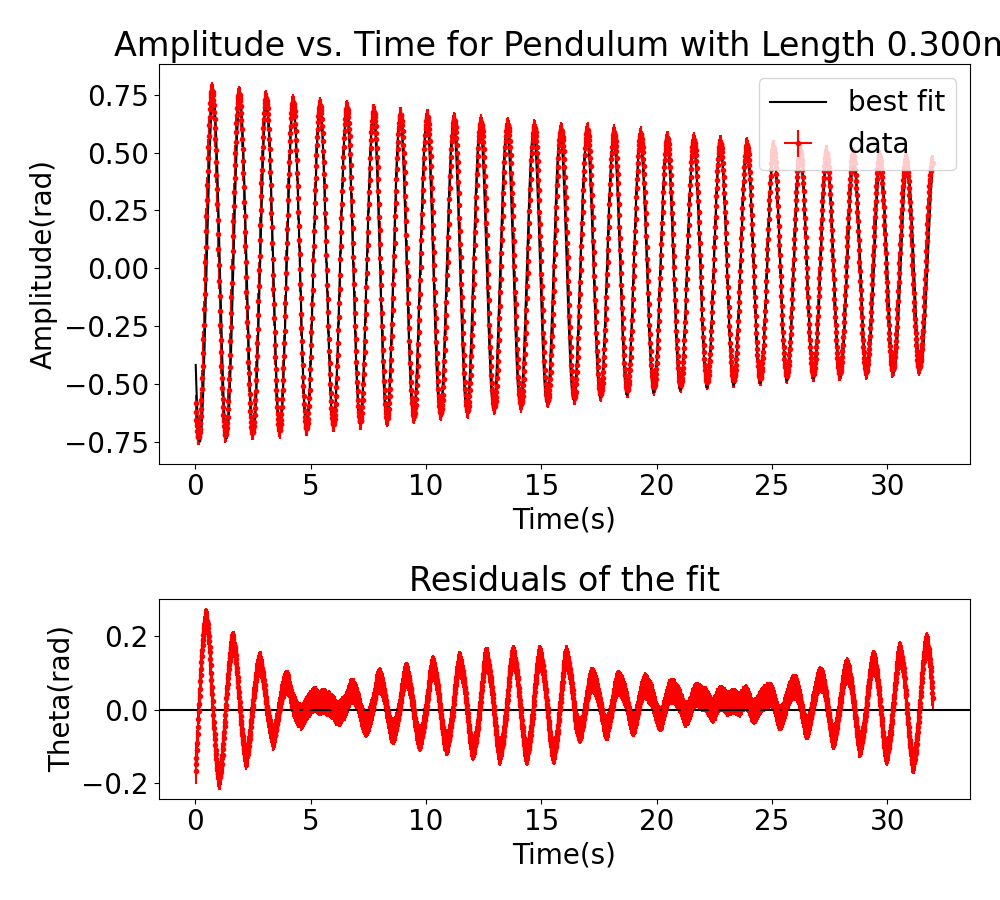
\includegraphics[width=8cm]{all_angle_graph.png}
        \caption*{\textbf{Figure 5.1:} Complete angle vs time graph obtained from  experimental result. It shows the amplitude of the pendulum decreases as time increases.}
    \end{figure}
    \begin{figure}[H]
    \centering
        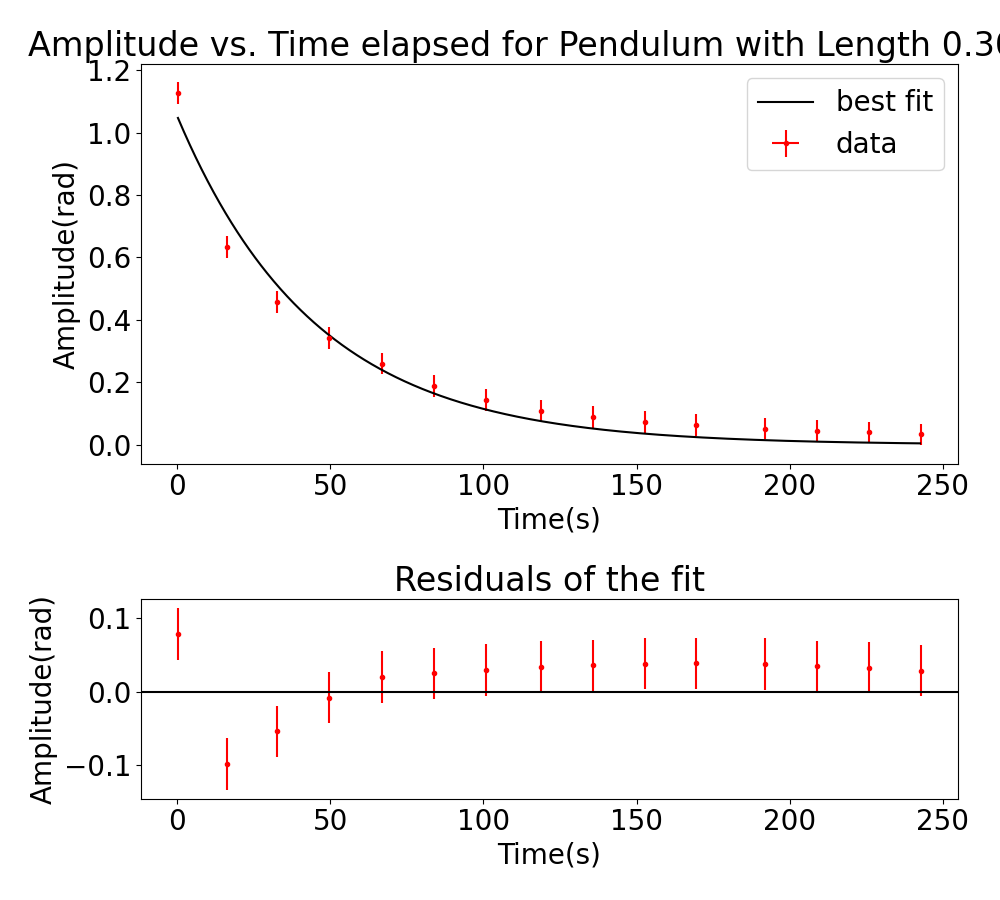
\includegraphics[width=8cm]{exp_graph.png}
        \caption*{\textbf{Figure 5.2:} Complete angle vs time graph obtained from  experimental result. It shows the amplitude of the pendulum decreases as time increases. It included the first two points, which decreased the accuracy.}
    \end{figure}

\section{Citation}
    \begin{enumerate}
    \item Wilson.B (2023) "PHY180 Lab Proiect 2023"  University of Toronto. \\ 
    https://q.utoronto.ca/courses/324650/files/27269654?//module;tem;d = 4893671
    \item Ivan.W (2023) "OpenCV Tracker"
    \item Design, B. (n.d.). DaVinci Resolve\&nbsp;18. DaVinci Resolve 18 | Blackmagic Design. \\https://www.blackmagicdesign.com/products/davinciresolve 
    \end{enumerate}


    


\end{document}
